\documentclass[10pt,a4paper,twocolumn]{article}

\usepackage{multicol}
\usepackage{amsbsy, amssymb, latexsym, amsmath, braket}
\usepackage[tiny]{titlesec}
\usepackage[hmargin=0.5cm,vmargin=0.7cm]{geometry}
\usepackage[utf8x]{inputenc}
\usepackage{polski}
\usepackage{scalefnt}
\usepackage[yyyymmdd,hhmmss]{datetime}
\usepackage{commath}
\usepackage{graphicx}

\graphicspath{ {./images} }

% Potrzebne do algorytmu Euklidesa.
\usepackage{tikz}
\usetikzlibrary{tikzmark}

\newcommand{\angles}[1]{\left\langle #1 \right\rangle}


\newcommand{\entry}{$\bullet$\hspace{0.15em}}
\newcommand{\subentry}{$\circledcirc$\hspace{0.15em}}
% https://tex.stackexchange.com/a/7045/80219
\newcommand{\textsubentry}[1]{\tikz[baseline=(char.base)]{
            \node[shape=circle,draw,inner sep=1pt] (char) {#1};\hspace{0.15em}}}

% Automatyczne generowanie listy liczby pierwszych:
% https://tex.stackexchange.com/a/134320/80219
\makeatletter
\def\primes#1#2{{%
  \def\comma{\def\comma{, }}%
  \count@\@ne\@tempcntb#2\relax\@curtab#1\relax
  \@primes}}
\def\@primes{\loop\advance\count@\@ne
\expandafter\ifx\csname p-\the\count@\endcsname\relax
\ifnum\@tempcntb<\count@\else
  \ifnum\count@<\@curtab\else\comma\the\count@\fi\fi\else\repeat
\@tempcnta\count@\loop\advance\@tempcnta\count@
\expandafter\let\csname p-\the\@tempcnta\endcsname\@ne
\ifnum\@tempcnta<\@tempcntb\repeat
\ifnum\@tempcntb>\count@\expandafter\@primes\fi}
\makeatother

\titlespacing{\section}{0pt}{0pt}{0pt}
\titlespacing{\subsection}{0pt}{0pt}{0pt}
\titlespacing{\subsubsection}{0pt}{0pt}{0pt}

% Wyłącz numerowanie stron.
\pagenumbering{gobble}

\setlength{\parindent}{0pt}
% Odległość pomiędzy liniami. Zmniejsz, jeżeli brakuje miejsca.
\setlength{\parskip}{0.5ex}

\title{Notatki ASD}

\begin{document}
% Rozmiar czcionki.
\scalefont{.48}

\text{\tiny{
    Wersja z \today\ o \currenttime\ (\pdfmdfivesum file{./karta-wzorow.tex})
}}

% Drzewiaste struktury danych
\section{Drzewiaste struktury danych}
\subsection{BST}
\entry
Drzewa wyszukiwań binarnych (drzewa BST – Binary Search Trees) - drzewa binarne, w których elementy
rozmieszczone są w porządku symetrycznym.

\entry
Właściwości BST:  

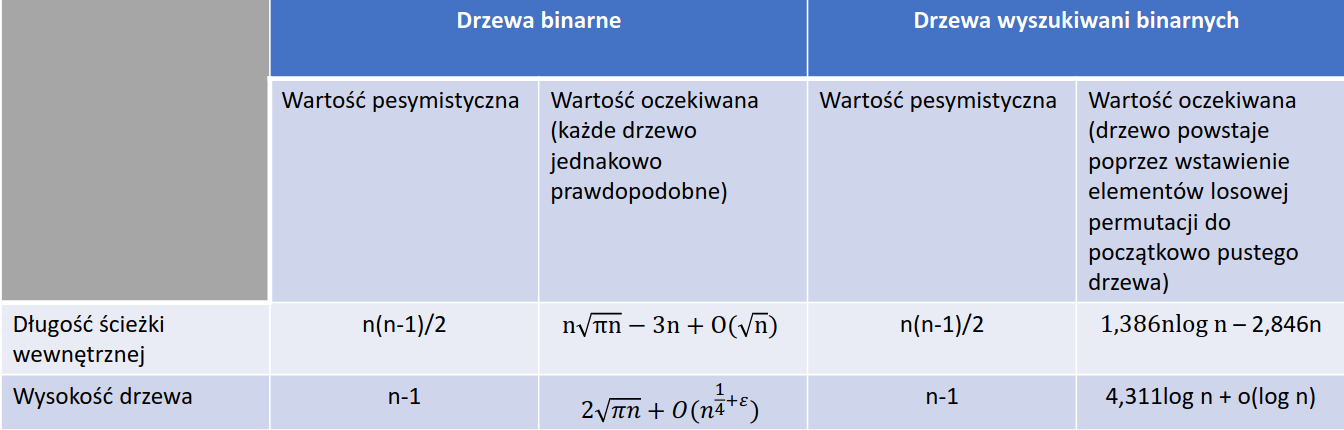
\includegraphics[scale=0.25]{drzewa1.png}

\subsection{AVL}
\entry
AVL-drzewo – drzewo wyszukiwań binarnych, w którym dla każdego węzła wysokości jego poddrzew
różnią się co najwyżej o 1

\entry
Złożoność operacji to $\log{n}$ gdzie n to wielkość drzewa.

\entry 
Atrybuty węzłów drzewa z wykładu:  

Key(v) – klucz  

Left(v), Right(v), Parent(v) – wskaźniki odpowiednio do lewego i prawego dziecka oraz rodzica  

Bf(v) – wskaźnik zrównoważenia (ang. balance factor) równy h(T(Left(v)) – h(T(right(v)) ∈ {-1, 0, 1}

\entry
Przyjmujemy, że węzeł zewnętrzny ma wysokość -1.

\entry
Rotacje zachowują porządek symetryczny w BST, numerację infiksową (inorder) węzłów drzewa binarnego!

\entry
Pojedyncza rotacja w prawo i lewo:  

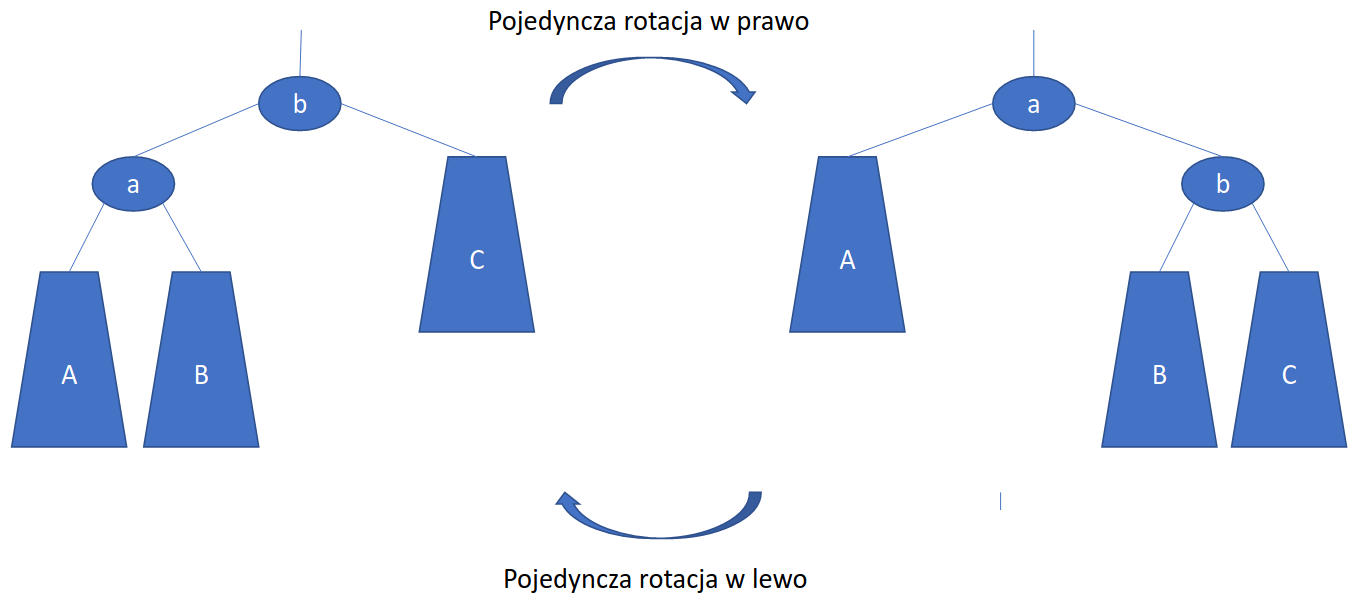
\includegraphics[scale=0.25]{pojedynczaRotacja.png}

\entry
Podwójna rotacja w prawo:  

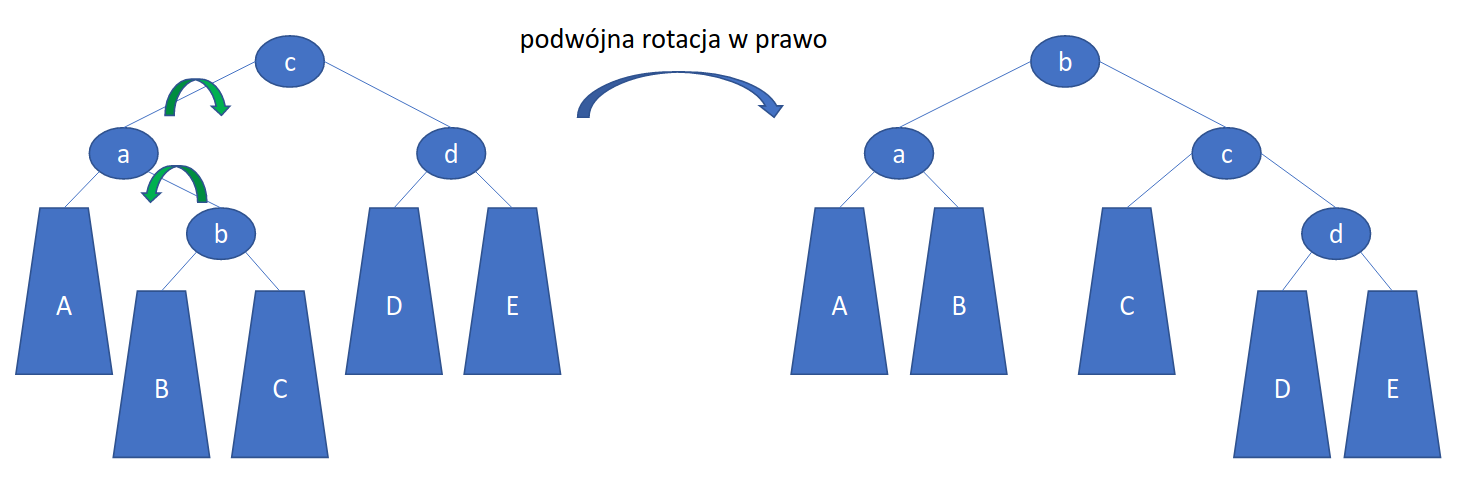
\includegraphics[scale=0.25]{podwojnaWPrawo.png}

\entry
Podwójna w lewo:

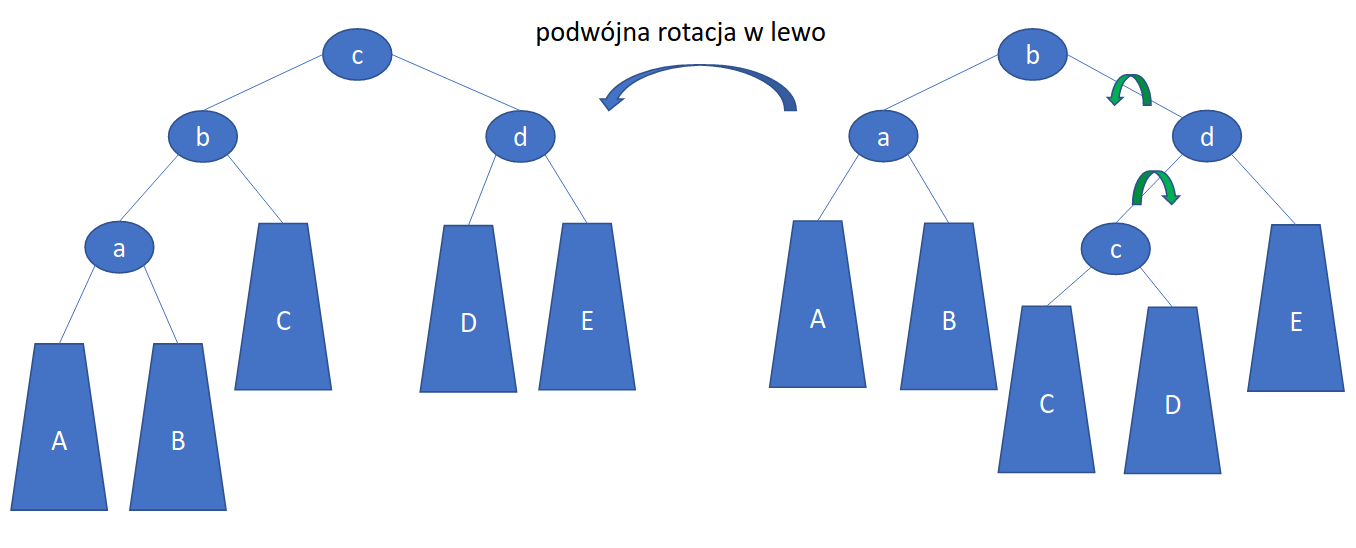
\includegraphics[scale=0.25]{podwojnaWLewo.png}

\entry
Schemat wstawiania elementu gdy urosło lewe poddrzewo(symetrycznie dla prawego):

Bf v = -1 $\Rightarrow$ Bf v = 0; STOP

Bf v = 0 $\Rightarrow$ Bf v = 1; $\Uparrow$ (poprawiaj w górę)

Bf v = 1 $\Rightarrow$ rotacja

\entry
Schemat usuwania elementu gdy zmalało lewe poddrzewo(symetrycznie dla prawego):

Bf v = −1 $\Rightarrow$ rotacja

Bf v = 0 $\Rightarrow$ Bf v = −1; STOP

Bf v = 1 $\Rightarrow$ Bf v = 0; $\Uparrow$ (poprawiaj w górę)

\entry
Wzbogacenia AVL przedstawione na wykładzie:

OnLeft(v) – liczba węzłów w lewym poddrzewie v

Max(v) – maksimum z elementów w poddrzewie o korzeniu v

\entry
Rotajce w drzewie zachowują kolejność infiksową(inorder)

\subsection{Splay}
\entry
Operacje na drzewach splay są w czasie zamortyzowanym logarytmicznym

\entry
Podczas każdej operacji na drzewie splay wierzchołek, na którym wykonujemy operację, staje się korzeniem.

\entry
Local Splay:

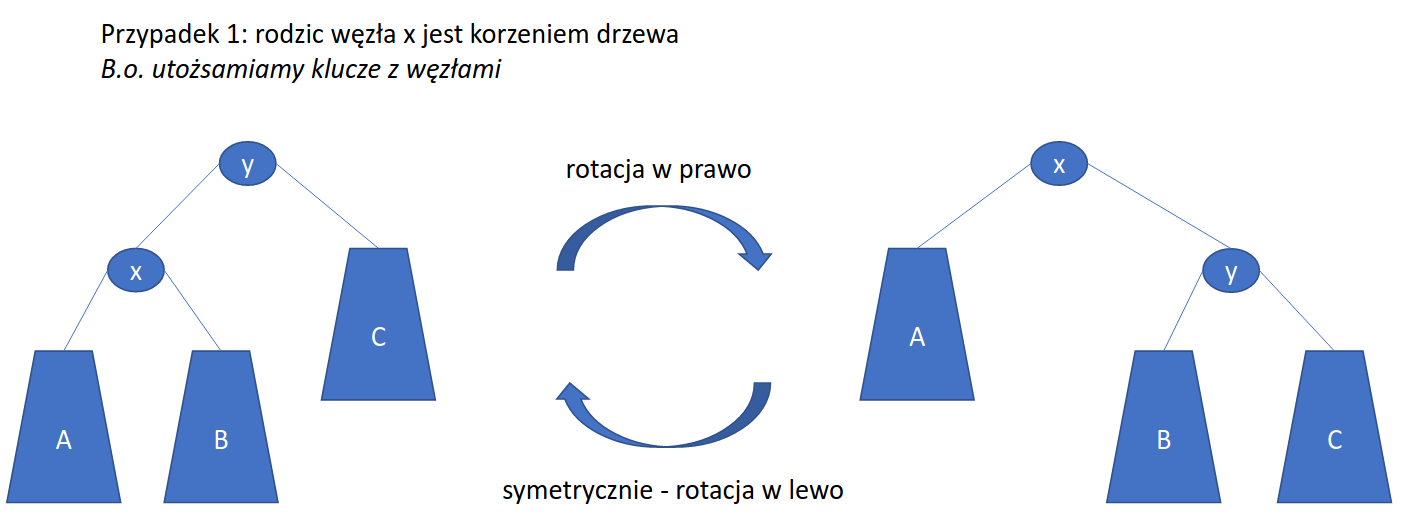
\includegraphics[scale=0.25]{splay1.png}

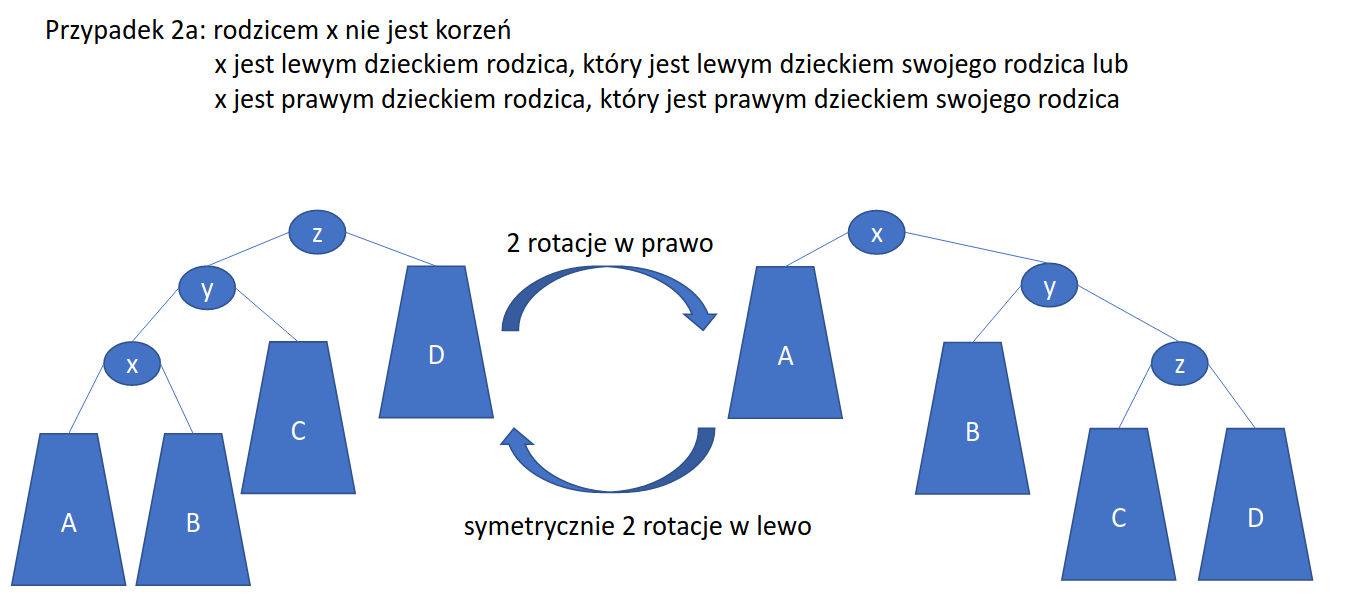
\includegraphics[scale=0.25]{splay2.png}

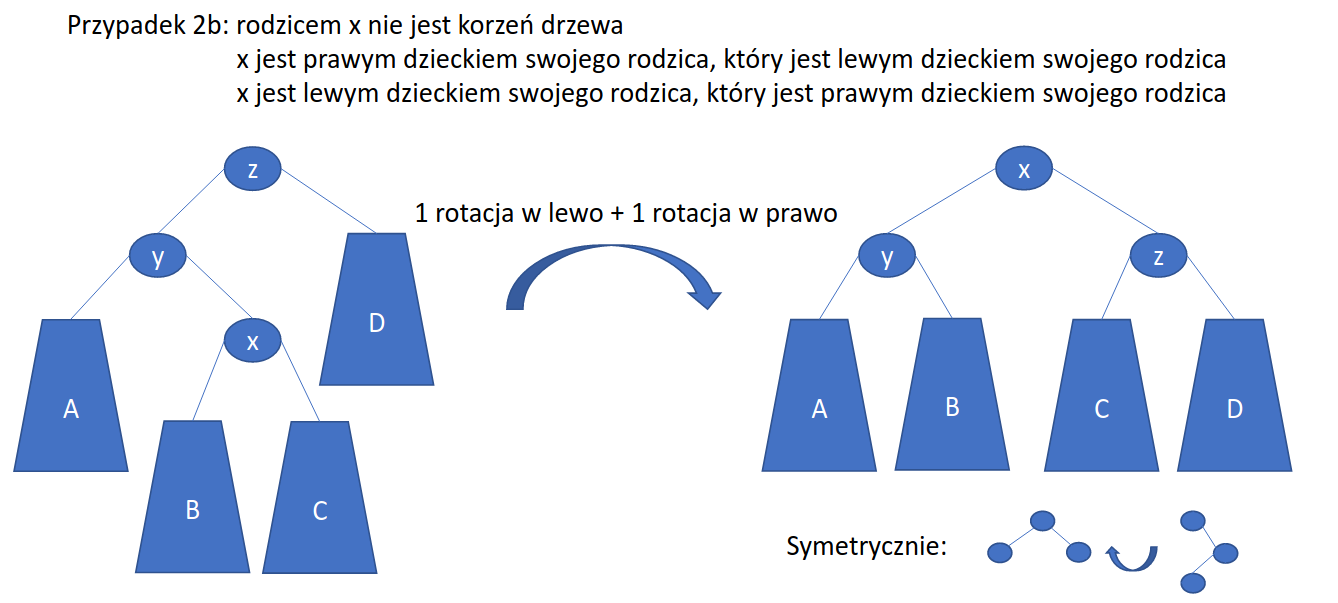
\includegraphics[scale=0.25]{splay3.png}

\entry 
Istnieje operacja split która dzieli drzewo na dwa poddrzewa według wieżchołka v. (lewe drzewo ma klucze mniejsze a prawe wieksze niż klucz v)

\subsection{Drzewa B}
\entry
Niech t będzie liczbą całkowitą większą od 1.

B-drzewem (minimalnego) stopnia t nazywamy drzewo z korzeniem spełniające poniższe warunki:

• Każdy węzeł x ma następujące atrybuty:

a) m – liczba kluczy aktualnie pamiętanych w x

b) m kluczy Key1, Key2, ..., Keym uporządkowanych rosnąco (załóżmy ponadto, że mamy
wirtualnych strażników Key0 = -∞ oraz Keym+1 = +∞)

c) Leaf – atrybut logiczny przyjmujący wartość TRUE wiw, gdy x jest liściem

• Każdy węzeł wewnętrzny x zawiera m+1 wskaźników P1, P2, ..., Pm+1 do swoich dzieci w drzewie.
Dla liści wartością tych wskaźników jest NULL.

• Każdy klucz K w poddrzewie wskazującym przez Pi spełnia warunek Keyi-1 < K < Keyi.

• Wszystkie liście leżą na tej samej głębokości równej wysokości drzewa h.

• Każdy węzeł różny od korzenia całego drzewa musi zawierać co najmniej t-1 i co najwyżej 2t-1
kluczy (odpowiednio, co najmniej t i co najwyżej 2t wskaźników do dzieci, o wartościach
równych NULL jeśli jest to liść).

• W niepustym drzewie korzeń musi zawierać, co najmniej 1 i co najwyżej 2t-1 kluczy (odpowiednio
co najmniej 2 i co najwyżej 2t wskaźników do dzieci - o wartościach NULL, jeśli jest to
jednocześnie liść).

\entry 
Złożoności

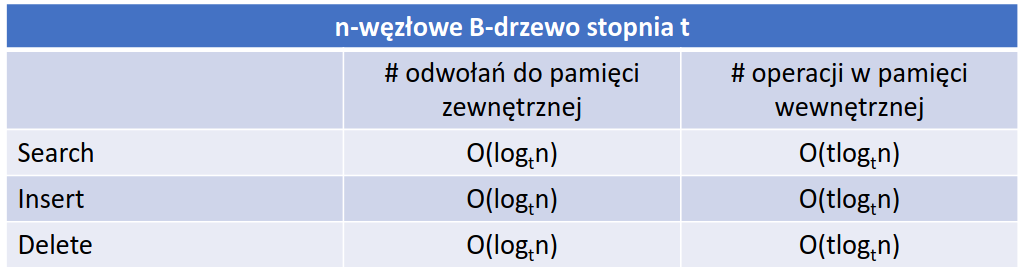
\includegraphics[scale=0.35]{boperacje.png}

\entry 
B-drzewo o (minimalnym) stopniu t = 2 nazywamy 2-3-4-drzewem (każdy węzeł, nie liść, ma 2 lub 3 lub 4 dzieci)

\entry
Korzeń poddrzewa do którego wchodzimy, różny od korzenia, nigdy nie jest minimalny!

\entry
Korzeń poddrzewa do którego wchodzimy nigdy nie jest maksymalny!

\entry
Wysokość drzewa: $h \leq \log_t(\frac{n+1}{2})$

\entry
Przykład drzewa

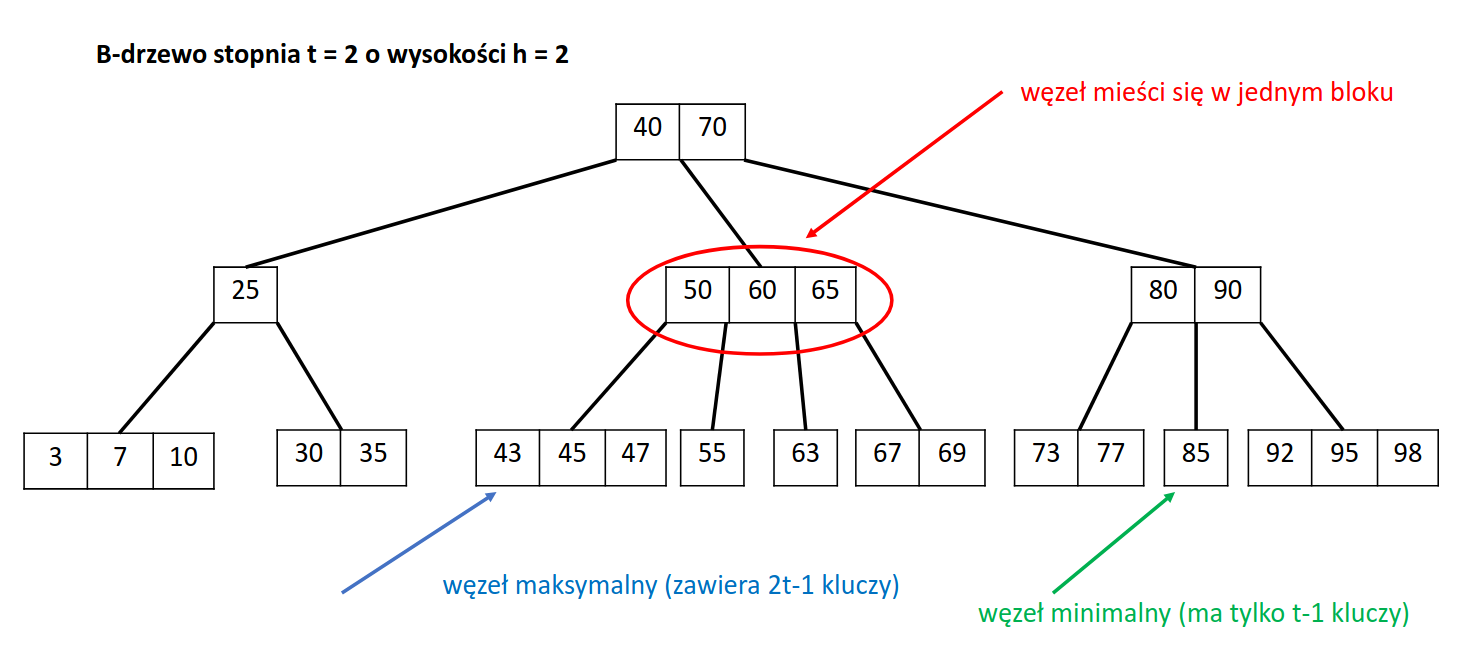
\includegraphics[scale=0.25]{bprzyklad.png}

\subsection{Drzewa Czerwono Czarne}

\entry
Drzewo czerwono-czarne – drzewo BST, w którym każdy węzeł jest pokolorowany
na czerwono lub czarno zgodnie z następującymi regułami:

1. korzeń drzewa jest czarny

2. każdy czerwony węzeł ma czarnego rodzica

3. każdy węzeł zewnętrzny (NULL) jest czarny

4. każda ścieżka (elementarna) z ustalonego węzła do węzła zewnętrznego w jego
poddrzewie zawiera tyle samo węzłów czarnych

\entry
Wysokość drzewa wynosi $h \leq 2 \log_2(\frac{n+1}{2})$

\entry
Slajdy

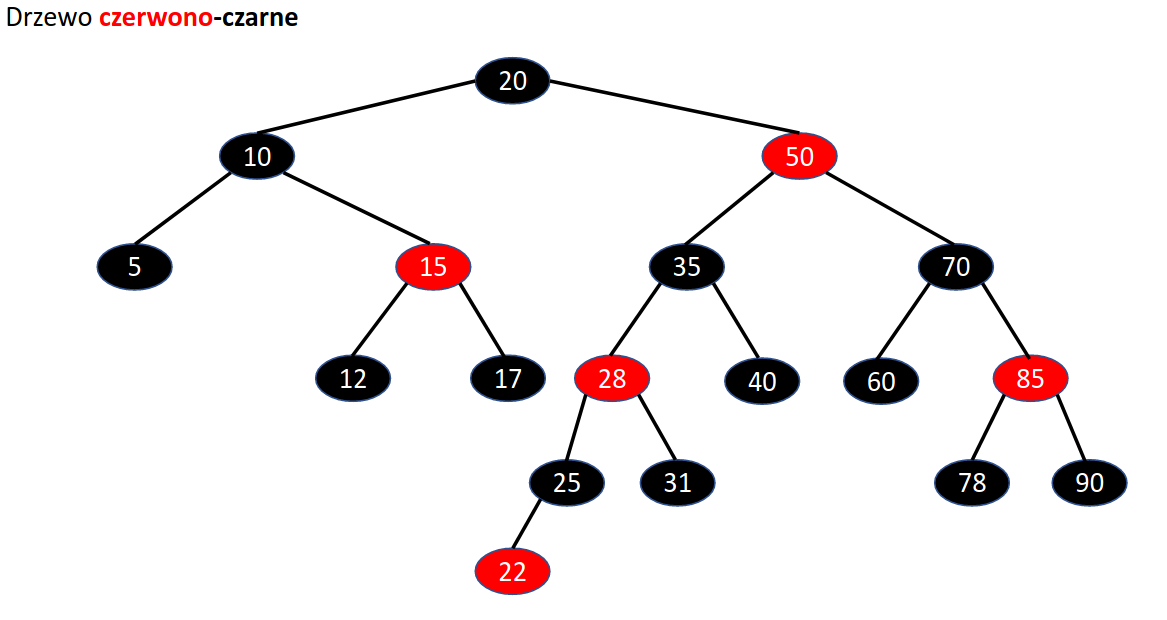
\includegraphics[scale=0.25]{cc1.png}

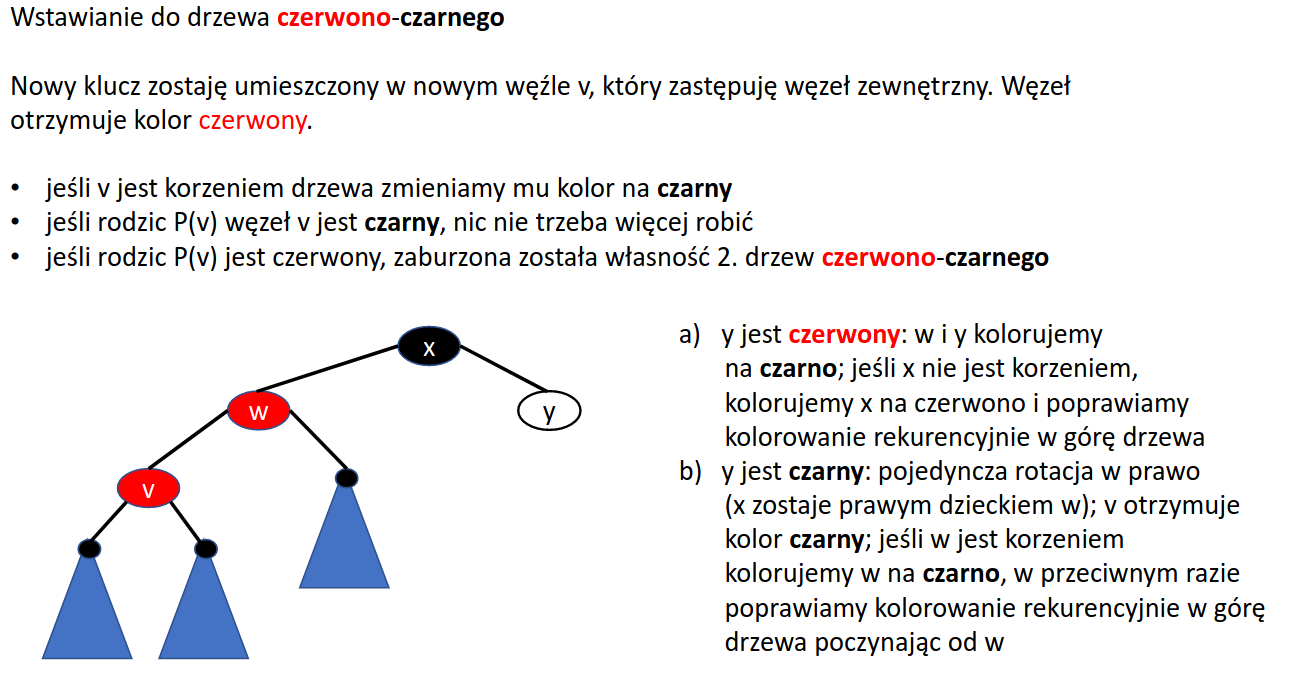
\includegraphics[scale=0.25]{cc2.png}

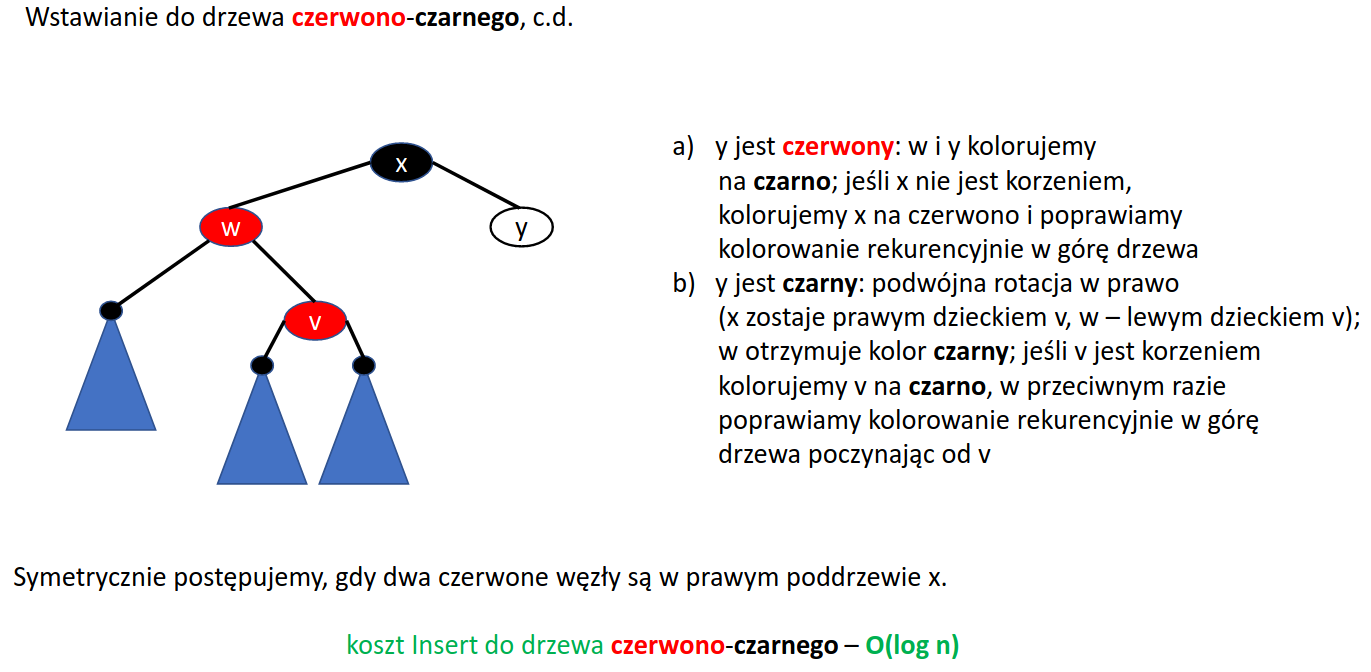
\includegraphics[scale=0.25]{cc3.png}

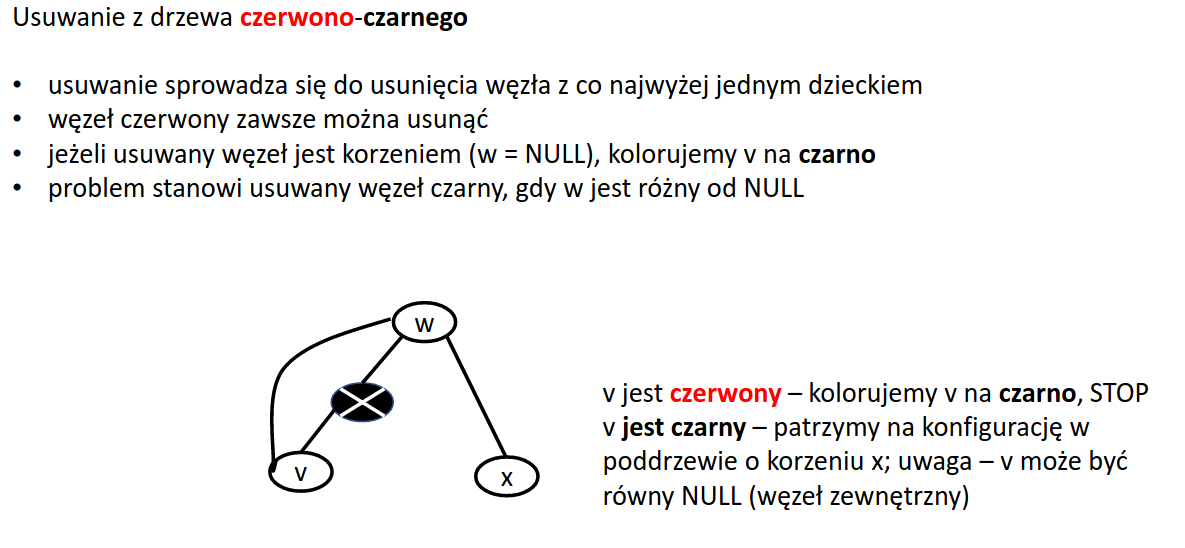
\includegraphics[scale=0.25]{cc4.png}

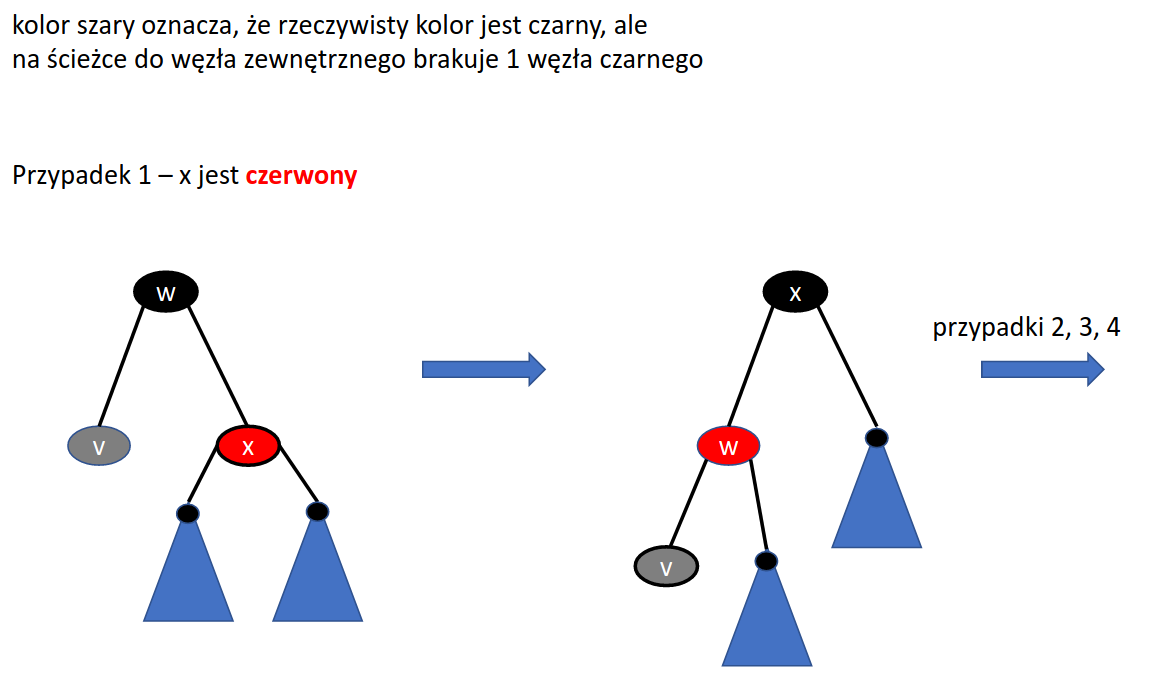
\includegraphics[scale=0.25]{cc5.png}

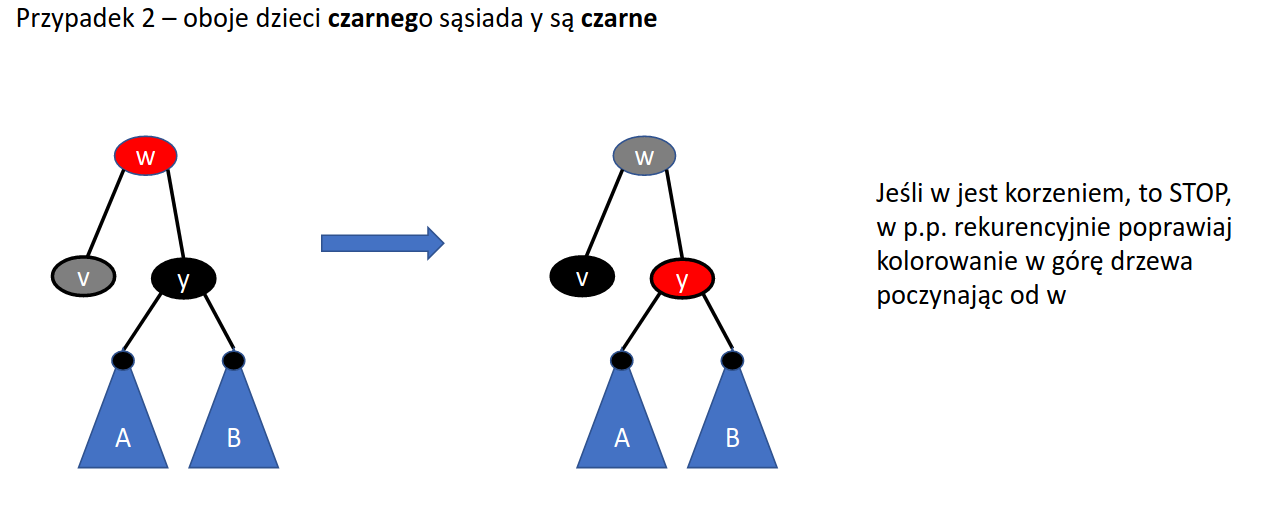
\includegraphics[scale=0.25]{cc6.png}

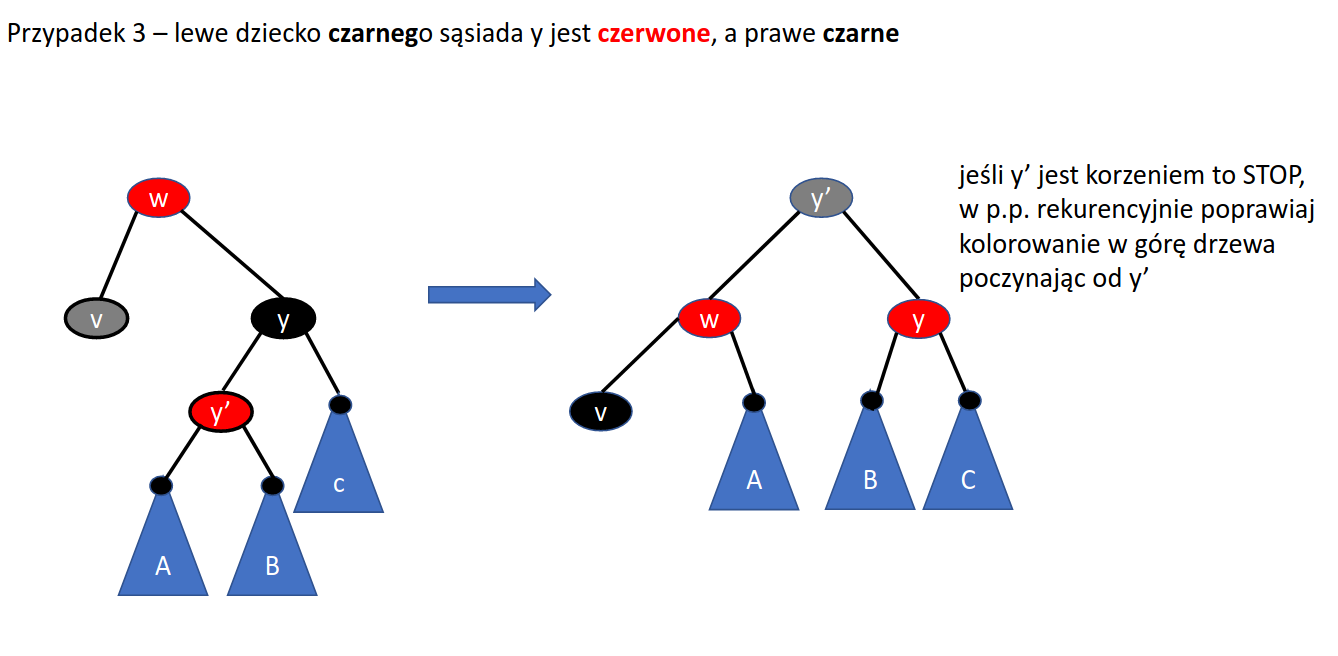
\includegraphics[scale=0.25]{cc7.png}

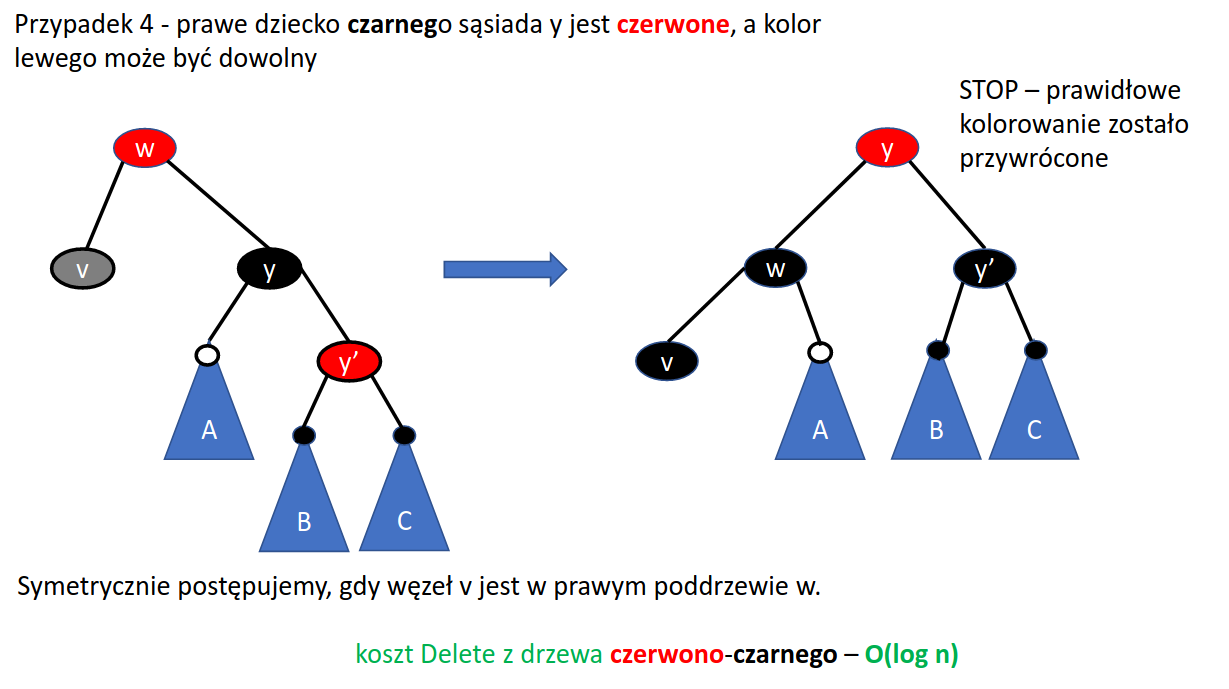
\includegraphics[scale=0.25]{cc8.png}


% Algorytmy grafowe
\section{Algorytmy grafowe}

\subsection{Algorytm Floyda-Warshalla}

\entry
Problem najlżejszych ścieżek pomiędzy wszystkimi
parami wierzchołków

\entry 
Idea:

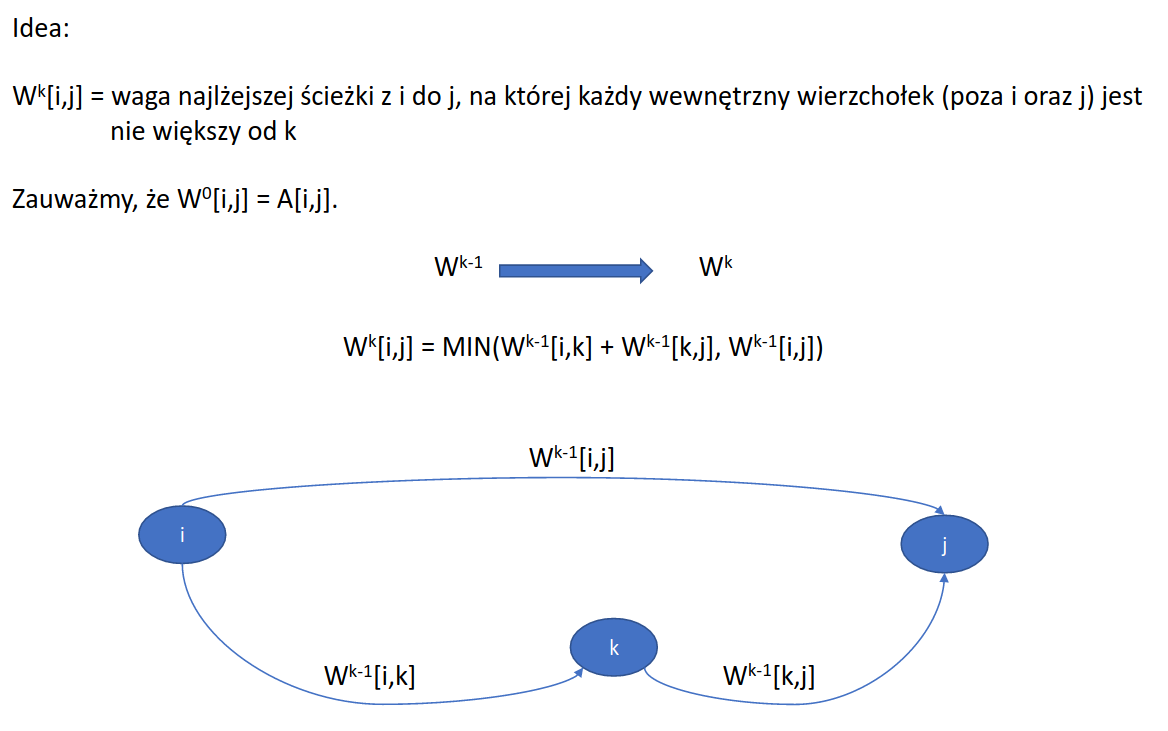
\includegraphics[scale=0.25]{ideawarszal.png}

\subsection{Spójne składowe}

\entry
Czas O(n+m) gdzie n to liczba wierzchołków a m liczba krawędzi.

\entry 
Dane

G=(V,E) – graf n-wierzchołkowy

Wynik

funkcja C: V →V taka, że C[u] = C[v] wtedy i tylko wtedy, gdy u i v są w tej samej spójne składowej

\subsection{Najkrótsze ścieżki}

\entry 
Czas O(n+m) gdzie n to liczba wierzchołków a m liczba krawędzi.

\entry 
Dane

G = (V,E) - graf spójny, n = $|V|$

s – wyróżniony wierzchołek w G

Wynik

D[1..n] – tablica, w której D[u] to długość najkrótszej ścieżki z wierzchołka s do wierzchołka u mierzona liczbą krawędzi

Metoda

przeszukiwanie grafu, w którym zbiór S implementujemy jako kolejkę FIFO (First In First Out)
jest to tzw. przeszukiwanie wszerz (ang. BFS – Breadth First Search)

\subsection{Przeszukiwanie wgłąb}
\entry
Własności

\entry
krawędź niedrzewowa łączy zawsze potomka z przodkiem w
w drzewie przeszukiwania w głąb

\entry
numer dfs wierzchołka jest zawsze większy od numeru dfs jego
właściwego przodka

\subsection{Dwuspójne}

\entry
Wierzchołek v w grafie G nazywamy rozdzielającym (punktem artykulacji), jeśli jego usunięcie z G
(wraz z incydentnymi z nim krawędziami) zwiększa liczbę spójnych składowych w G.

\entry 
mostem w grafie G nazywamy krawędź, której usunięcie zwiększa liczbę spójnych składowych grafu.

\entry
spójny graf G jest grafem dwuspójnym wierzchołkowo (krawędziowo), jeśli nie zawiera wierzchołków
rozdzielających (mostów)

\entry
Dwuspójną składową grafu G nazywamy każdy jego maksymalny dwuspójny podgraf (z maksymalną możliwą liczbą
wierzchołków i krawędzi).

\entry 
Istnieje algorytm znajdowania liczby dwuspójnych w grafie w czasie O(n+m) za pomocą funkcji low

\entry
Struktura dwuspójny składowych

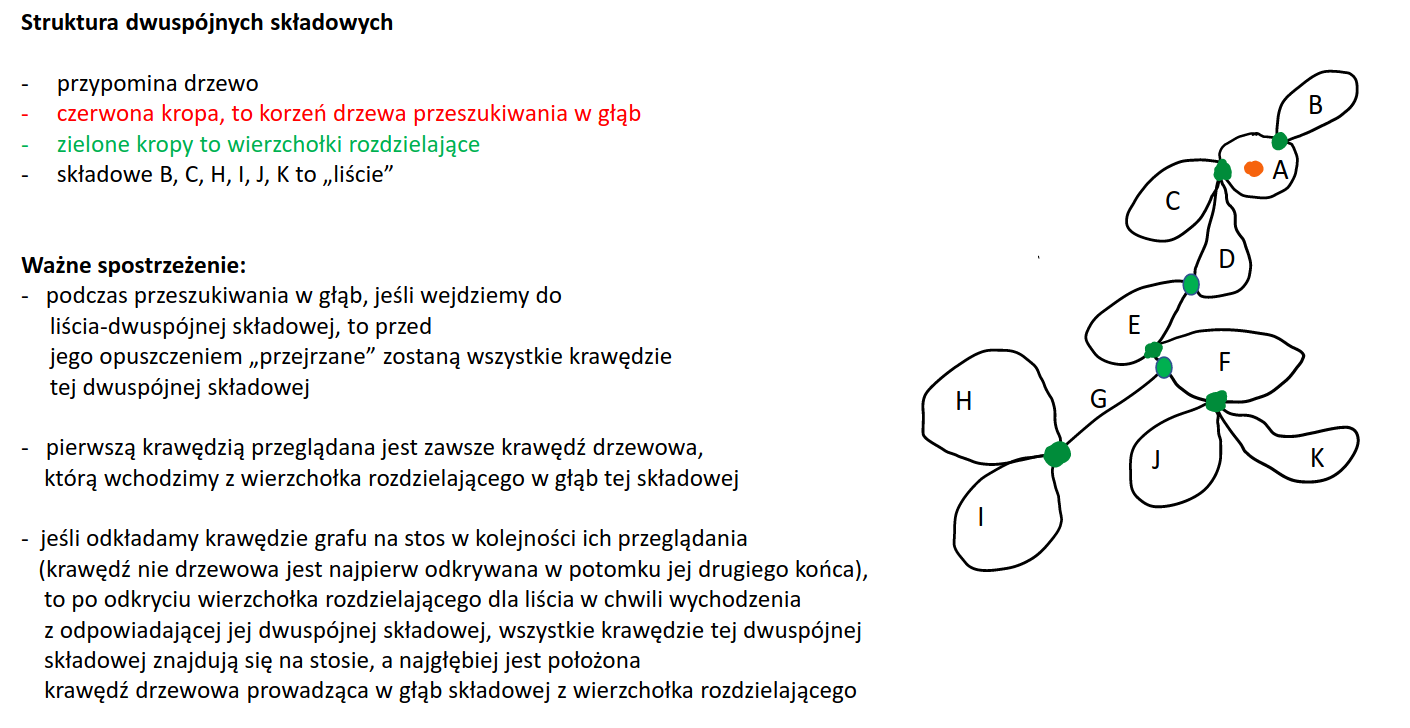
\includegraphics[scale=0.25]{sdwuspoj.png}

\entry
Istnieje algorytm znajdowania dwuspójnych składowych w czasie O(m)


% Kolorowanie
\section{Kolorowanie}

\entry
Kolorowaniem (wierzchołkowym) grafu nieskierowanego nazywamy takie przypisanie kolorów
wierzchołkom grafu, że żadne dwa sąsiednie wierzchołki nie mają przypisanych tych samych kolorów.

\entry
Jeżeli istnieje kolorowanie grafu G z użyciem k kolorów, to mówimy że G jest k-kolorowalny.

\entry
Minimalną liczbę kolorów, którymi można pokolorować graf G nazywamy jego liczbą chromatyczną i
oznaczamy przez $\chi$  G 

\entry
Przez $\Delta $(G) oznaczamy maksymalny stopień wierzchołka w grafie G (stopień wierzchołka to liczba
jego sąsiadów w tym grafie)

\entry
Oczywiste: $\chi$ G ≤ $\Delta $(G) + 1.

\subsection{Brooks}

\entry
Każdy graf G różny od cyklu nieparzystej długości i grafu pełnego można pokolorować $\Delta $(G) kolorami.

\entry
Graf jest k-kolorowalny wtedy i tylko wtedy, gdy każda jego dwuspójna składowa jest k-kolorowalna.

\entry
Algorytm kolorowania Brooksa+ działa w czasie O(n+m)

\entry
Slajd:

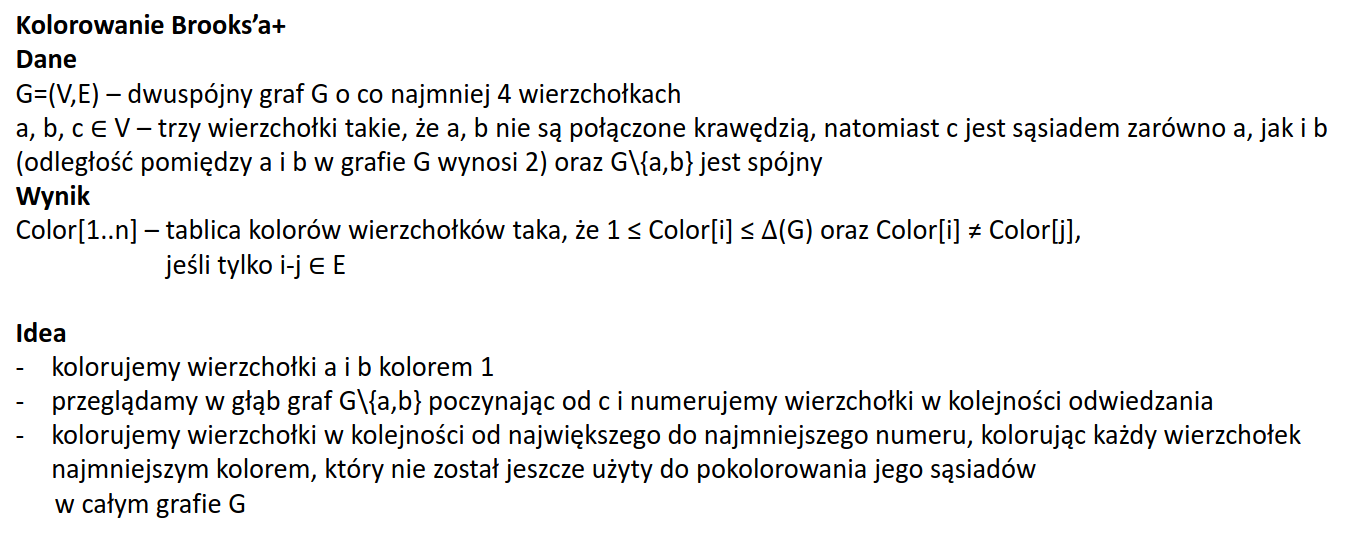
\includegraphics[scale=0.25]{boorks+.png}


\end{document}
